\documentclass[11pt,a4paper]{article}
%-----------------------------------
%% Geometry and layout
\usepackage[
  margin=1.8cm,
  includefoot,
  bmargin=0.9cm,
  footskip=0.9cm
]{geometry}

\linespread{1.15}

\usepackage{float}
\setcounter{topnumber}{2}
\setcounter{bottomnumber}{2}
\setcounter{totalnumber}{4}
\renewcommand{\topfraction}{0.85}
\renewcommand{\bottomfraction}{0.85}
\renewcommand{\textfraction}{0.15}
\renewcommand{\floatpagefraction}{0.8}
\renewcommand{\textfraction}{0.1}
\setlength{\floatsep}{5pt plus 2pt minus 2pt}
\setlength{\textfloatsep}{5pt plus 2pt minus 2pt}
\setlength{\intextsep}{5pt plus 2pt minus 2pt}

%-----------------------------------

\usepackage[T1]{fontenc}
\usepackage{lmodern}

\newcommand{\supth}{\textsuperscript{th}\ }

%-----------------------------------
\usepackage{xcolor}
\usepackage[colorlinks]{hyperref}
%\usepackage[hyperpageref]{backref}
\usepackage{breakurl}
\hypersetup{
    colorlinks=true,       % false: boxed links; true: colored links
    linkcolor=orange,          % color of internal links
    citecolor=magenta,        % color of links to bibliography
    filecolor=magenta,      % color of file links
    urlcolor=cyan,           % color of external links
    runcolor=cyan
}
%-----------------------------------
\usepackage{graphicx}% Include figure files
\graphicspath{{./figures/}}
\usepackage[font={small}]{caption}
\usepackage{wrapfig}


\usepackage{physics}

%===================================
\begin{document}
\title{MBEA: Maximal Biclique Enumeration Algorithm, Implementation in C++}
\author{Danial Dervovic}
\date{\today}

\maketitle
% !TEX root = ./report.tex
Bipartite graphs are used in multiple problem domains to represent the relationships between pairs of disparate data types.
Interpreting these relationships is often achieved by enumerating the maximal bicliques in a given bipartite graph, a computationally challenging task.
Zhang \emph{et al.} provide the most efficient currently known algorithm~\cite{Zhang2014} for carrying out this task.
In fact, they give two slightly different algorithms.
This report describes the implementation of these two algorithms for MPHYG002, coursework 1.

\section{Background}

Now let us look at the problem in detail.
A \emph{bipartite graph} is a graph whose vertices can be partitioned into a pair of non-empty, disjoint partitions such that no two vertices in the same partition are connected by an edge.
Let $G= (U\cup V, E)$ be a bipartite graph, with $U$ and $V$ denoting its two vertex set partitions, and $E$ denoting its edge set.
A bipartite graph $G$ can be described by its $\abs{U}\times \abs{V}$ \emph{biadjacency matrix}, $A_G$, with elements defined as follows
\begin{equation}\label{eq:biadjacency}
    [A_G]_{i,j} = \begin{cases}
    1, & \text{iff $(i,j)\in E$};\\
    0, & \text{otherwise};
\end{cases}
\qq{for all $i\in U,\ j \in V$}. 
\end{equation}
A \emph{biclique} $C = (U', V')$ is a subgraph of $G$ induced by a pair of disjoint subsets $U'\subseteq U$, $V' \subseteq V$, such that for all $u\in U'$, $v \in V'$, $(u,v)\in E$.
More informally, a biclique in $G$ is a fully connected subgraph of $G$.
A \emph{maximal biclique} $C = (U',V')$ in $G$ is a biclique for which there is no additional vertex in $V\cup U$ which you can add to $C$ and it still remain a biclique.

\begin{wrapfigure}{r}{0.5\textwidth}
    \centering
    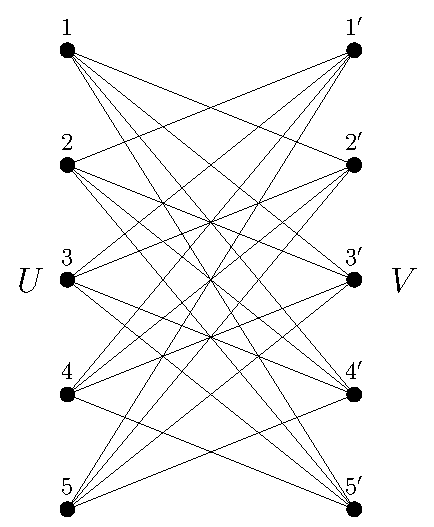
\includegraphics[width=0.25\textwidth]{crown}
    \caption{
    A crown graph on ten vertices.
    There are $2^{5}-2 = 30$ maximal bicliques in this graph.
    For every subset of $U$ (apart from $\emptyset$ and $U$ itself), the induced subgraph is a unique maximal biclique. 
    }
    \label{fig:crown}
\end{wrapfigure}

The problem we are interested in is the enumeration of all the maximal bicliques in a given bipartite graph $G$.
This problem is intrinsically computationally hard since in some cases, the number of maximal bicliques in a bipartite graph can be exponential in the number of vertices.
An example of such a graph is the \emph{crown graph}, an example of which is shown in Figure~\ref{fig:crown}.
For any crown graph on $2n$ vertices, there are $2^n - 2$ maximal bicliques.

The algorithms by Zhang \emph{et al.} are called the (improved) Maximum Biclique Enumeration Algorithm, or iMBEA and MBEA respectively.
MBEA roughly works by recursively choosing subsets of one of the vertex partitions and checking if the induced subgraph is a biclique and if this biclique is maximal.
iMBEA is essentially the same as MBEA, but takes actions to prune the recursion tree of paths which won't lead to maximal bicliques and to decrease the lengths of paths which do.
The detailed algorithms can be seen in~\cite[Algorithm: MBEA]{Zhang2014}.

\section{Implementation}

The C++ program written for this work, implementing both MBEA and iMBEA is called \texttt{MBEA}.
It is a command line program which takes as input the location of a text file and a parameter to decide between MBEA and iMBEA.
The text file should contain the biadjacency matrix of a graph.
The program then prints a list of the maximal bicliques in the graph, according to the vertex labelling implicitly defined by the input biadjacency matrix, as well as the total number of maximal bicliques.   
This list is printed to \texttt{stderr}, so can be piped to other programs through the command line in the usual way.

\subsection{The End User and Environment}

The form the program is presented in naturally assumes the user is familiar with the command line, specifically a UNIX-like terminal.
The program needs to be built by the user on their machine, but since \texttt{MBEA} uses CMake as a build system and has few dependencies, this should be straightforward.
Furthermore, the explicit procedure required is specified in the build instructions in \texttt{README.md}, which anyone who has used a terminal should be familiar with.
The usage instructions for \texttt{MBEA} itself are (hopefully!) explicit enough that anyone with a passing familiarity with bipartite graphs should be able to use \texttt{MBEA} with few issues.

The program has been built and tested on Mac OSX 10.12.2 with both clang-802.0.41 and gcc 6.3.0 separately, using CMake version 3.7.2.
In theory, this should work in the same way for Linux also.
Windows support could be added with CMake, but unfortunately time constraints prevented addition of this feature.

\subsection{Code Design}

The real strength of the iMBEA and MBEA algorithms over competing algorithms within this problem domain is that they explicitly take advantage of the bipartite graph structure.
With this in mind, my first consideration was to see if the \texttt{Boost::Graph} library could be of any use.
Unfortunately, this library has little in the way of class structure and algorithms explicitly for bipartite graphs.
Because of this, I chose to use my own class, \texttt{BipartiteGraph} to represent a bipartite graph.

A bipartite graph in essence is two sets of vertices and their adjacency relations.
For the vertices, I created a \texttt{Vertex} class.
Adjacency was represented by a \texttt{std::shared\_ptr} to another \texttt{Vertex} object.
Care was taken so that for a given edge in $E$, both \texttt{Vertex} objects had the other as a neighbour.
The smart pointer was used to help prevent memory leaks.
Then each vertex partition was represented by an \texttt{std::vector<std::shared\_ptr<Vertex>{>}}.
In fact, I provide a wrapper class \texttt{VertexSet} around this data type, to easily facilitate adding to and removing vertices from a set of vertices, a fundamental operation in the MBEA algorithm.

\texttt{BipartiteGraph} also has the child class \texttt{Biclique}, which is natural since every biclique is a bipartite graph, but not the other way round.
The MBEA and iMBEA algorithms are implemented in the \texttt{BicliqueFinder} class.
The strategy pattern was used to easily switch between the iMBEA and MBEA algorithms easily.
I use the class \texttt{CommandLineParser} to parse the input from the command line.
Ideally some kind of Command Line Interface framework would have been preferable to use, as it would be more extensible, but this seemed overly complex for a project of this size.

\subsection{Testing}

I used the Googletest framework for testing, primarily because my IDE has full support for it.
The test coverage is fairly comprehensive in terms of the classes.
However, I would have liked more time to try more test cases per method.
For the tests of the algorithm itself and regression tests I chose to primarily use crown graphs, as they have the maximum possible number of maximal bicliques for a given number of vertices.
Further to this, the MBEA and iMBEA algorithms  must traverse their respective whole recursion trees to be seen to be functioning properly.
Since for a crown graph, every node in the recursion tree gives a maximal biclique, correctly reporting the maximal bicliques in this case is a good indicator that the implementation is correct.


\section{Experiments}

To show an example of the code working, I ran a runtime comparison between MBEA and iMBEA, which they do (on a much larger scale) in~\cite{Zhang2014}.
This experiment code is in \texttt{report/experiments/generate} \texttt{\_experimental\_data.py} and the results were plotted using \texttt{report/experiments/plot\_experimental\_} \texttt{data.py}.
\par
More precisely, the algorithm was ran on generated Erd\H{o}s-R\'{e}nyi random bipartite graphs.
An Erd\H{o}s-R\'enyi random bipartite graph $G(m,n,p)$ has $\abs{U} = m$, $\abs{V} =n$ and for each pair $(i,j)$ for all $i\in U$, $j\in V$ the edge $(i,j)$ exists with probability $p$.
Erd\H{o}s-R\'enyi random bipartite graphs $G(m,n,p)$ were generated with the values $\abs{U} = \{7, 11, 16, 19\}$, $\abs{V} = \{10, 15, 20, 25\}$ and $p=\{0.1, 0.5, 0.75, 0.9\}$, with 20 graphs generated for each $(m,n,p)$ combination.
The runtime for MBEA and iMBEA are plotted against the number of vertices for various $p$ in Figure~\ref{fig:plots}. 

\begin{figure}
    \centering
    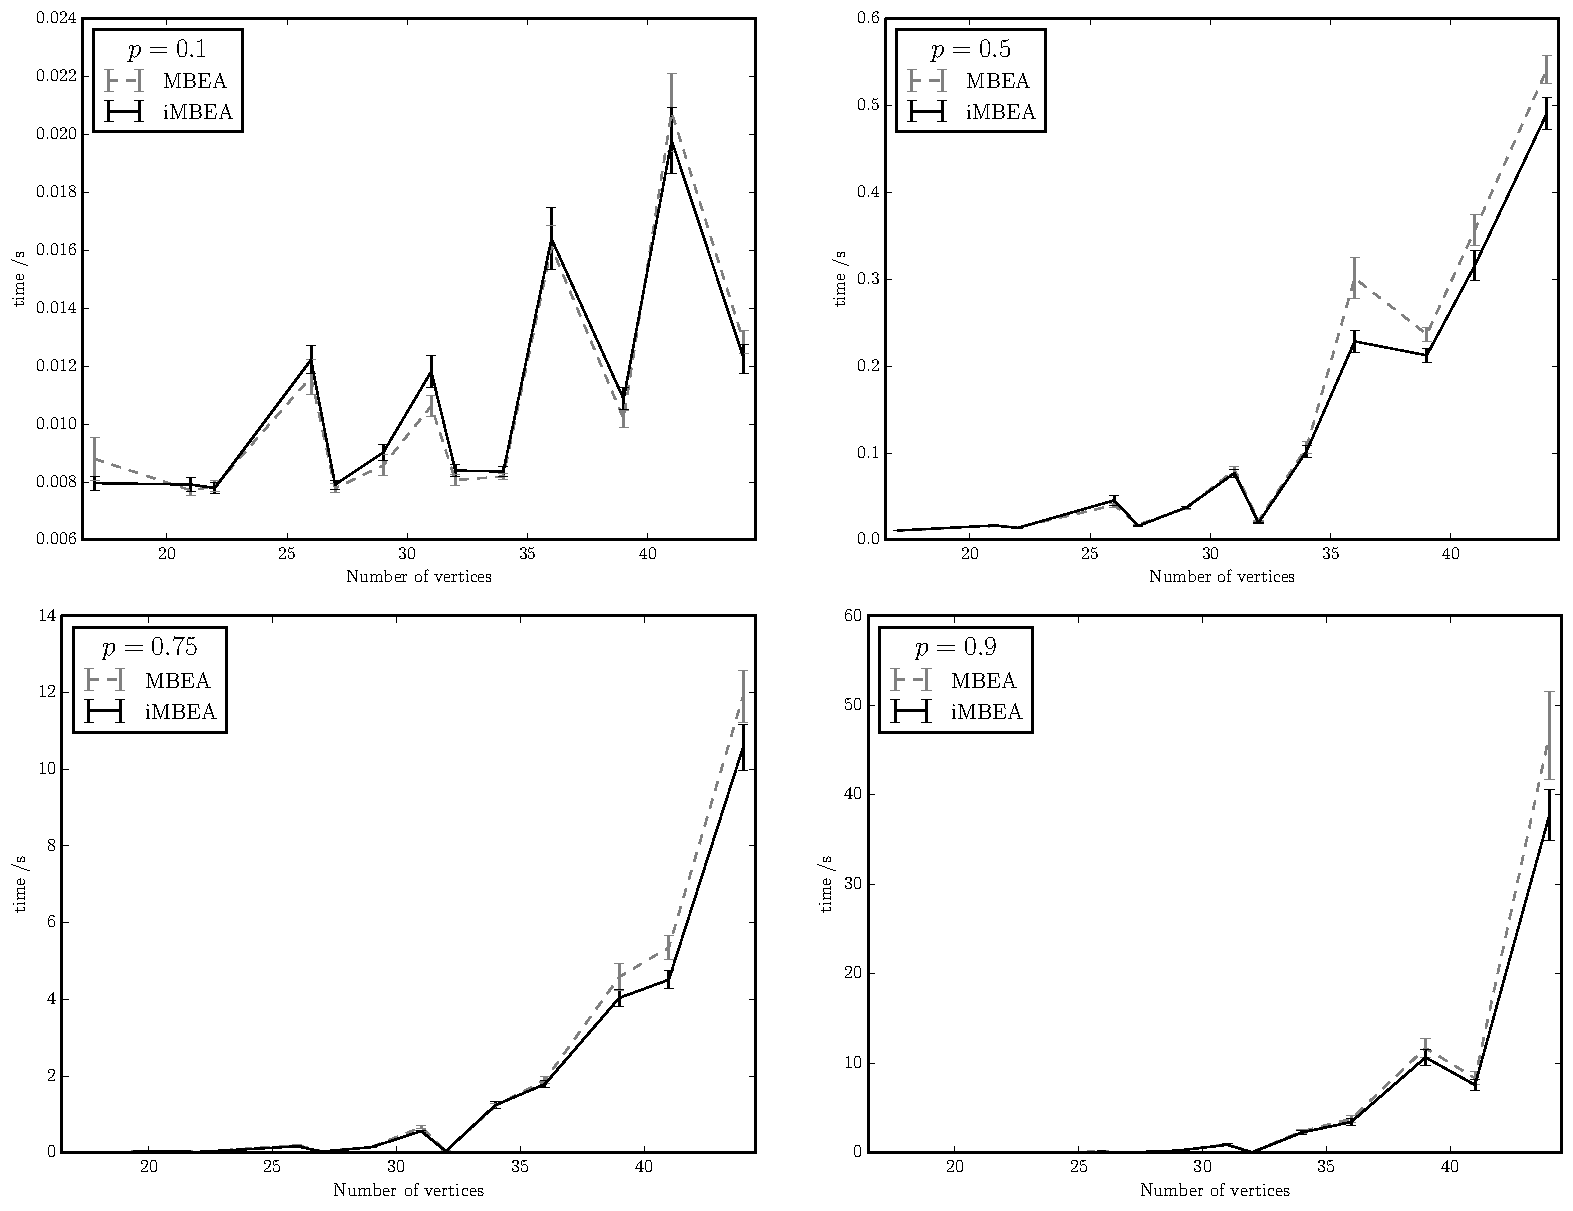
\includegraphics[width=0.95\textwidth]{plots}
    \caption{
    Results of experiment comparing implementations of MBEA and iMBEA.
    Note that in general, iMBEA runs faster, as one would expect from~\cite{Zhang2014}.
    Also note that as $p$ increases, i.e. the graphs get denser, the overall runtime increases.
    Error bars are standard error on the mean.
    }
    \label{fig:plots}
\end{figure}


Observe that in general, iMBEA is faster than MBEA as expected.
An exception to this is in the $p=0.1$ where the graphs are more sparse.
iMBEA comes in to its own with the more dense graphs.
Also note that for dense graphs (with $p$ close to $1$) that the runtime starts approaching a minute for graphs on 45 vertices.

\section{Conclusions}

Due to the nature of the problem itself, this code probably can't scale to arbitrary bipartite graphs with an enormous number of vertices.
This behaviour is reported in~\cite{Zhang2014} and is suggested by Figure~\ref{fig:plots}.
For substantial speedup in the sense of making the runtime subexponential, the algorithm itself would need to be parallelised, with a large number of workers executing the algorithm.

A design improvement I'd like to implement would be more flexible input.
Whilst the code is robust to incorrect input and provides the appropriate warnings, ideally a user would want more options for how to input data.
An example would be an adjacency list of vertices with string labels.
This could probably be implemented with a modest amount of templating.


\bibliographystyle{nicebib-alpha}
\bibliography{refs.bib}
\end{document}
